\section{Quality Requirements}

\subsection{Quality Tree}

\begin{figure}[H]
    \centering
    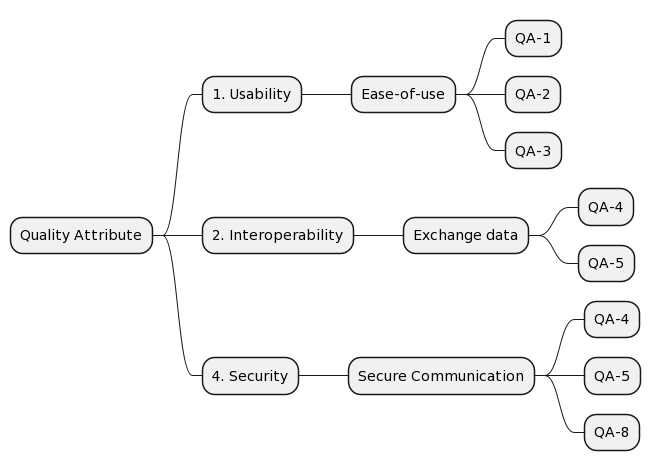
\includegraphics[width=0.7\textwidth]{assets/quality_tree.png}
    \caption{Preliminary functions}
    \label{fig:preliminary_use_case}
\end{figure}


\subsection{Evaluation Scenarios} 
From the requirements, \ref{Requirement_Overview}, we could develop the following uses cases and depict the main quality 
attributes of this project. 

\begin{table}[H]
    \setstretch{1.0}
    \begin{tabularx}{\textwidth}{lX}
    \toprule
    Use Case & Description  \\
    \midrule
    UC-1: Register as \gls{client} & The \gls{client} registers an e-mail address.\\
    UC-2: Login & The \gls{client} logins in to the system. \\
    UC-3: Places an order & The \gls{client} chooses a \gls{provider}. \\
    UC-4: Register payment & The \gls{client} registers a payment method. \\
    UC-5: Register as \gls{provider} & The \gls{provider} registers their facility and products. \\
    UC-6: Update availability & The \gls{provider} uploads their product catalog. \\
    \bottomrule
    \end{tabularx}
\end{table}

With the following use cases we will  be able to define the major quality attributes that are involved in the 
development of this application. They should be measurable and testable so we can verify if the system meets 
the needs our \glsplural{stakeholder} \cite{refbook:DSHC}.

\begin{table}[H]
    \setstretch{1.0}
    \begin{tabularx}{\textwidth}{lcXc}
        \toprule
        ID & Quality Attribute & Scenario & Associated Use Case  \\
        \midrule
        QA-1 & Usability & A \gls{provider} is able to register his company, to specify the kind of products he/she offers 
        and upload a logo or picture of his shop and products in a easy and fast (within 5 Minutes) fashion. & UC-5 \\
        QA-2 & Usability & A \gls{provider} is able to update the offers at any time. &  UC-6 \\
        QA-3 & Usability & A \gls{client} is able to search and filter options. &  UC-6 \\
        QA-4 & Interoperability & A \gls{client} can register his e-mail using another account (Google, Microsoft, Facebook)
        in a \gls{federated login} & UC-1 \\
        QA-5 & Interoperability & A \gls{client} can pay the order using a \gls{mobile payment gateway} (e.g. Stripe, Square, PayPay, 
        SecurePay) & UC-4 \\
        QA-5 & Performance & A \gls{client} registers his/her e-mail address and can immediately browse in the app. & UC-1 \\
        QA-6 & Performance & A \gls{client} opens the app and he can immediately search for products or \glsplural{provider}. & UC-2 \\
        QA-7 & Performance & A \gls{client} chooses a \gls{provider} and places his order. After the confirmation
        of payment, a push-message is displayed in the app confirming the purchase. & UC-3 \\
        \bottomrule
    \end{tabularx}
\end{table}

\newpage
The defined quality attributes are represented in the following scenarios:


\begin{table}[H]
    \begin{tabularx}{\textwidth}{|c|X|}
        \hline
        \multicolumn{2}{c}{\textbf{Usability}} \\
        \hline
        \toprule
        \multicolumn{1}{c}{Scenario} & \multicolumn{1}{c}{Value} \\
        \midrule
        Source & \gls{provider} \\
        Stimulus & wants to register his/her shops \\
        Artifact & app \\
        Environment & working time, during afternoon \\
        Response & offer available in the app \\
        Response Measure & How long did the registration and upload process take? How many and what kind of error messages
        did the \gls{provider} get?\\
         & \\
        Source & Registered \gls{provider} \\
        Stimulus & wants wants to make a last minute offer \\
        Artifact & app \\
        Environment & peak period, between 4 and 7 pm on Friday \\
        Response & immediate availability of the offer in the app \\
        Response Measure & How long did it take to upload an offer? How many and what kind of error messages did the 
        \gls{provider} get? \\
        & \\
        Source & Registered \gls{client} \\
        Stimulus & wants to search/filter offers \\
        Artifact & app \\
        Environment & peak period, between 4 and 7 pm on Friday \\
        Response & display of the filter/search output \\
        Response Measure & What kind of inputs did the user has to place until he/she finds what he/she wants?
        Did he have to type anything or were filter/search options available? How long it takes until the client
        finds a product? \\
        \bottomrule
    \end{tabularx}
\end{table}


\begin{table}[H]
    \begin{tabularx}{\textwidth}{|c|X|}
        \hline
        \multicolumn{2}{c}{\textbf{Interoperability}} \\
        \hline
        \toprule
        \multicolumn{1}{c}{Scenario} & \multicolumn{1}{c}{Value} \\
        \midrule
        Source & \gls{client} \\
        Stimulus & wants register using a \gls{federated login} \\
        Artifact & app and \gls{federated login} provider  \\
        Environment & peak period (on the context of the \gls{federated login} provider)\\
        Response & authentication succeed or failed\\
        Response Measure & How much data was transmitted and how much was queued? \\
        Focus & System overload \cite{refart:MKMS} \\
        & \\
        Source & \gls{client} \\
        Stimulus & wants to pay using existing mobile payment account \\
        Artifact & app and \gls{mobile payment gateway}  \\
        Environment & peak period (on the context of the gateway)\\
        Response & confirmation / declined \\
        Response Measure & Total amount generated data in the app that are transferred and processed and rejected
        by the gateway \\
        Focus & Connectivity and System overload \cite{refart:MKMS} \\
        \bottomrule
    \end{tabularx}
\end{table}

\begin{table}[H]
    \begin{tabularx}{\textwidth}{|c|X|}
        \hline
        \multicolumn{2}{c}{\textbf{Performance}} \\
        \hline
        \toprule
        \multicolumn{1}{c}{Scenario} & \multicolumn{1}{c}{Value} \\
        \midrule
        Source & \gls{client}  \\
        Stimulus & wishes to create an account \\
        Artifact & app \\
        Environment & weekend between 3 and 7 PM \\
        Response & immediate access to the app \\
        Response Measure & time between confirmation and access \\
         & \\
        Source & \gls{client}  \\
        Stimulus & wants to search for a \gls{provider} \\
        Artifact & app \\
        Environment & peak period, between 6 and 7 pm on a Friday \\
        Response & immediate access to the offers \\
        Response Measure & how quickly does the client's device get update of availabilities \\
        & \\
        Source & \gls{client}  \\
        Stimulus & places an order \\
        Artifact & platform \\
        Environment & peak period, between 6 and 7 pm on a Friday \\
        Response & confirmation of payment / payment declined \\
        Response Measure & How long did take until the client get the confirmation/declined of payment?\\
        \bottomrule
    \end{tabularx}
\end{table}

